\documentclass[xcolor={x11names}]{beamer}
\input{flat-blue-theme.inc}
\input{footnotes.inc}

\usepackage[T1]{fontenc}
\usepackage[utf8]{inputenc}
\usepackage[ngerman,english]{babel}
\usepackage[english]{datetime2}
\usepackage{microtype}
\usepackage{csquotes}

%
% TikZ
%
\usepackage{tikz}
\usetikzlibrary{
	arrows,
	arrows.meta,
	calc,
%	external,
	fadings,
	intersections,
	patterns,
	positioning,
	snakes
}
%\tikzexternalize[prefix=tikz-cache/]

\tikzset{every path/.append style={line width=0.5pt}}
\tikzset{every path/.append style={>=stealth'}}
\tikzset{
	between/.style args={#1 and #2}{
		at = ($(#1)!0.5!(#2)$)
	}
}
\tikzset{
	dot/.style={circle,fill,inner sep=0.4mm,outer sep=0.25mm}
}
% [params] pos id
\newcommand{\tikzDot}[3][]{\node (#3) at #2 [dot,#1]{};}

%
% BibTex
%

% Must be placed here before BibTeX and URL/ref related packages:
\PassOptionsToPackage{obeyspaces}{url} % Allow spaces in URLs
\PassOptionsToPackage{spaces}{url}     % Enable line breaks in URLs

\usepackage[toc, page]{appendix}
\usepackage[
	backend=bibtex8,
	style=numeric,
	sorting=none,
	urldate=long,
	backref
]{biblatex}
\usepackage{hyperref}
\usepackage[noabbrev]{cleveref}

\addbibresource{sources.bib}
\let\oldCite\cite
\renewcommand{\cite}[2][]{ \oldCite[#1]{#2}} % Add space before citation

\NewBibliographyString{diplomathesis}
\DefineBibliographyStrings{english}{
	diplomathesis = {diploma thesis},
}

%
% Commands
%

\newcommand{\bigo}[1]{\mathcal{O}(#1)}
\renewcommand{\n}{\hfill\\[0.5ex]}
\newcommand{\nn}{\hfill\\[2ex]}

% Environment to center content of a figure without adding extra spacing before the caption
\newenvironment{figcenter}
{%
	\parskip=0pt%
	\par%
	\nopagebreak%
	\centering%
}%
{%
	\par%
	\noindent%
	\ignorespacesafterend%
}

%
% Styling, Layout
%

\setbeamercovered{invisible}
\beamertemplatenavigationsymbolsempty
\condensedToc

% Remove subsection bar
\defbeamertemplate*{headline}{miniframes theme no subsection}
{%
	\begin{beamercolorbox}[colsep=1.5pt]{upper separation line head}
	\end{beamercolorbox}
	\begin{beamercolorbox}{section in head/foot}
		\vskip-5pt\insertnavigation{\paperwidth}\vskip5pt
	\end{beamercolorbox}%
	\begin{beamercolorbox}[colsep=1.5pt]{lower separation line head}
	\end{beamercolorbox}
}

\defbeamertemplate{description item}{align left}{\insertdescriptionitem\hfill}

%
% Metadata
%

\title[Master's thesis -- Colloquium]{A Hybrid Algorithm for Finding Shortest Paths Between Arbitrary Coordinates using a Combination of Network and Geometric Routing}
\author{Hauke Stieler}
\institute[Universität Hamburg -- Databases and Information Systems]{
	Universität Hamburg\\
	Faculty of Mathematics, Informatics and Natural Sciences\\
	Department of Informatics\\
	Databases and Information Systems
}
\date{\today}
\titlegraphic{
\includegraphics[width=0.3\textwidth]{../thesis/images/UHH-Logo_2010_Farbe_CMYK.pdf}}

\begin{document}
	{
		\setbeamertemplate{headline}{}
		\setbeamertemplate{footline}{}
		\vspace*{-0.65cm}
		\maketitle
		\addtocounter{page}{-1}
	}
	
	\begin{frame}[t]{Inhalt}
		\tableofcontents[hidesubsections]
	\end{frame}
	
	\section{Motivation}
	
		\begin{frame}{Realistic pedestrian routing}
			Beneficial for\n
			\begin{itemize}
				\item real-world end-user applications\\\textrightarrow\ indoor navigation, campus navigation
				\pause
				\item higher level applications\\\textrightarrow\ isochrones, walkability analysis
				\pause
				\item \textbf{agent-based simulations}\\\textrightarrow\ crowd behavior in evacuation scenario
			\end{itemize}
		\end{frame}
	
		\begin{frame}{Routing techniques}
			Graph-based:\n
			\begin{itemize}
				\item graph with edges representing roads / ways
				\item well optimized: Dijkstra, A*, speedup techniques
				\item detailed attributes in edges
				\pause
				\item only vertices are reachable\ \textrightarrow\ unable to traverse open spaces
			\end{itemize}
			\nn
			\pause
			Geometric routing:\n
			\begin{itemize}
				\item shortest path in presence of obstacles (i.e. lines and polygons)
				\item two strategies:
				\begin{itemize}
					\item graph generation (e.g. visibility graphs) + graph-based routing
					\item continuous Dijkstra
				\end{itemize}
				\pause
				\item path realism heavily depends on data quality
			\end{itemize}
		\end{frame}
	
		\begin{frame}{Example: Pure graph-based routing}
			\begin{figure}[t]
				\begin{figcenter}
					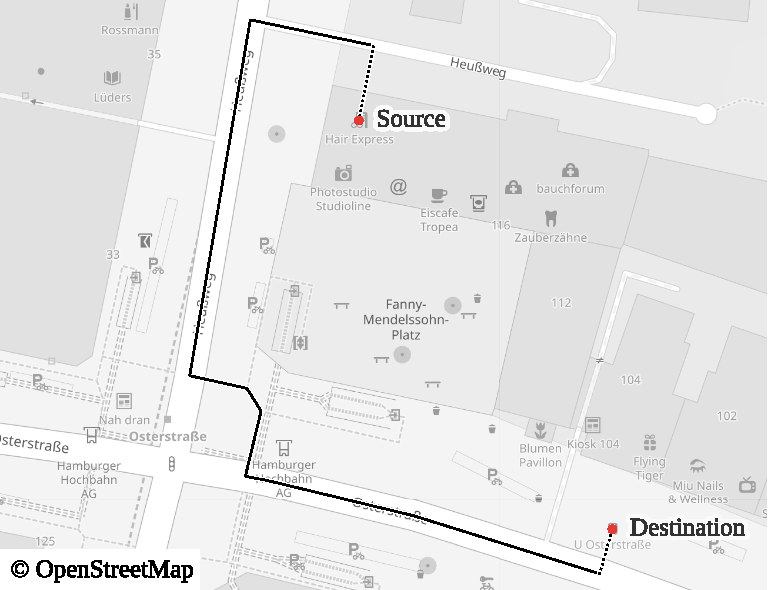
\includegraphics[width=0.65\textwidth]{images/qgis-routing-osterstrasse_routing.pdf}
				\end{figcenter}
				\caption{Graph-based routing result using \href{https://www.osm.org/directions?engine=graphhopper\_foot\&route=53.57657,9.95210;53.57601,9.95268}{\emph{GraphHopper}}.}
			\end{figure}
		\end{frame}
		
		\begin{frame}{Example: Expected routing behavior}
			\begin{figure}[t]
				\begin{figcenter}
					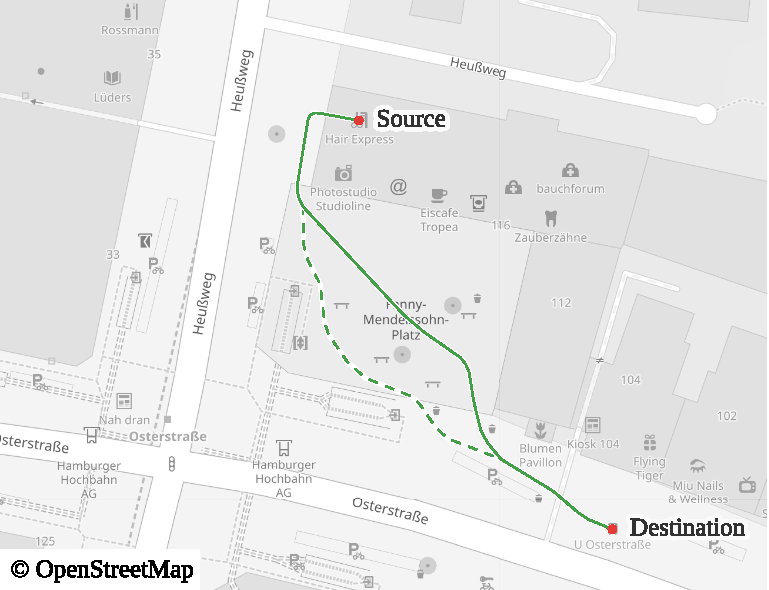
\includegraphics[width=0.65\textwidth]{images/qgis-routing-osterstrasse_expected.pdf}
				\end{figcenter}
				\caption{Routes an actual pedestrian would likely choose.}
			\end{figure}
		\end{frame}
		
%		\begin{frame}{Example 2: Densely built-up areas}
%			\begin{figure}[t]
%				\begin{figcenter}
%					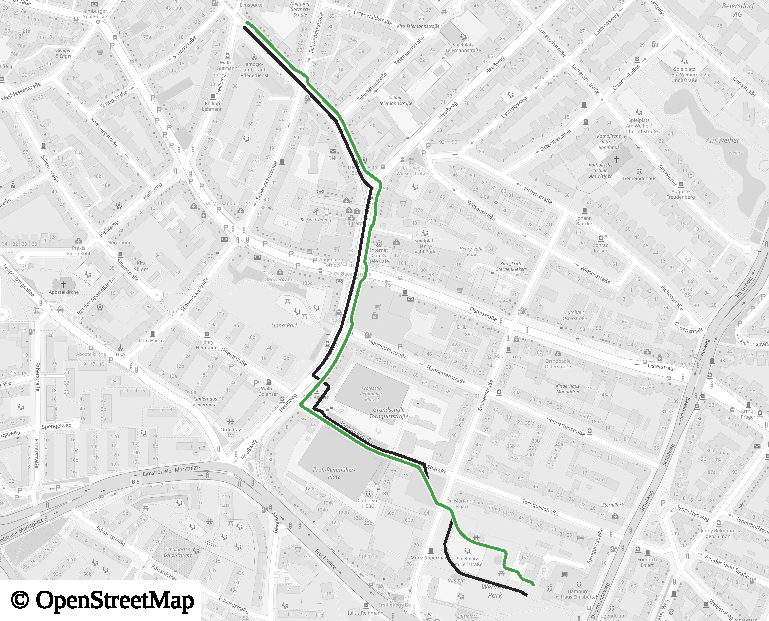
\includegraphics[width=0.65\textwidth]{images/qgis-routing-similar.pdf}
%				\end{figcenter}
%				\caption{Expected routes often follow graph edges, which hold valuable information.}
%			\end{figure}
%		\end{frame}
		
		\begin{frame}{Value of graph data}
			Graph data is still valuable:\n
			\begin{itemize}
				\item detailed information
				\begin{itemize}
					\item surface conditions, access restrictions, allowed vehicle types
				\end{itemize}
				\item definitely walkable
				\begin{itemize}
					\item no real-world obstacles in the way
				\end{itemize}
				\item sometimes without alternatives
				\begin{itemize}
					\item bridges, tunnels
					\item paths through obstacles (e.g. building passages)
				\end{itemize}
			\end{itemize}
		\end{frame}
	
	\section{Design}
	
		\begin{frame}{Wanted routing algorithm}
			Should be able to\n
			\begin{itemize}
				\item traverse open spaces\ \textrightarrow\ reach arbitrary locations
				\item use roads and ways
				\item create more realistic routes than purely graph-based routing
			\end{itemize}
			\nn
			\pause
			Additional requirements:\n
			\begin{itemize}
				\item based on C\# / .NET and MARS (Multi-Agent Research and Simulation)
				\item low impact on simulation time
			\end{itemize}
		\end{frame}
		
		\begin{frame}{Design decisions}
			Decisions of implemented algorithm:\n
			\begin{itemize}
				\item visibility graph generation
				\item merge with existing road network
				\item connect source / destination with visibility edges
				\item usage of graph-based routing
			\end{itemize}
			\nn
			\pause
			Alternative approaches:\n
			\begin{itemize}
				\item alternating routing with continuous Dijkstra
				\item merge of route segments in postprocessing step
				\item other graph-generation methods
				\begin{itemize}
					\item Voronoi diagrams, skeletonization
					\item ad-hoc generation (e.g. by using continuous Dijkstra)
				\end{itemize}
			\end{itemize}
		\end{frame}
		
		\begin{frame}{Components}
			\begin{figure}[t]
				\begin{figcenter}
					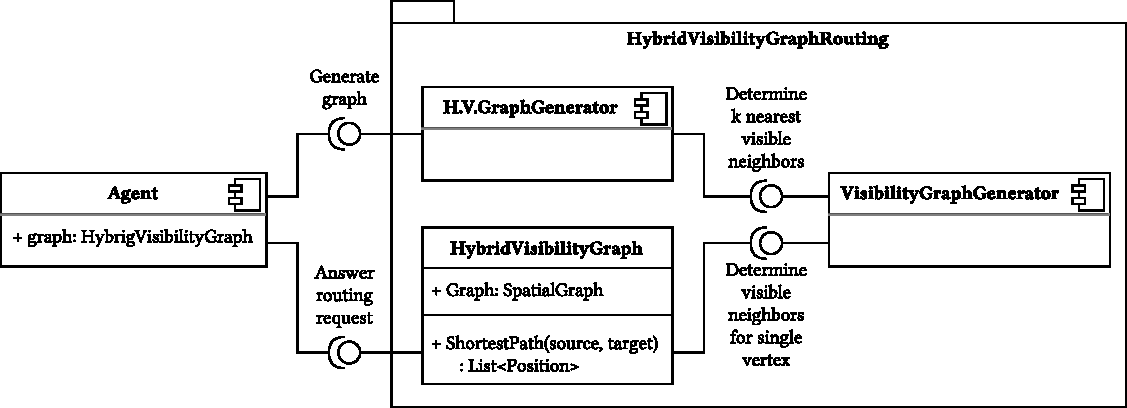
\includegraphics[width=0.95\textwidth]{images/components.pdf}
				\end{figcenter}
				\caption{Components of the implemented hybrid routing algorithm.}
			\end{figure}
		\end{frame}
		
		\begin{frame}{Graph generation}
			\begin{figure}[t]
				\begin{figcenter}
					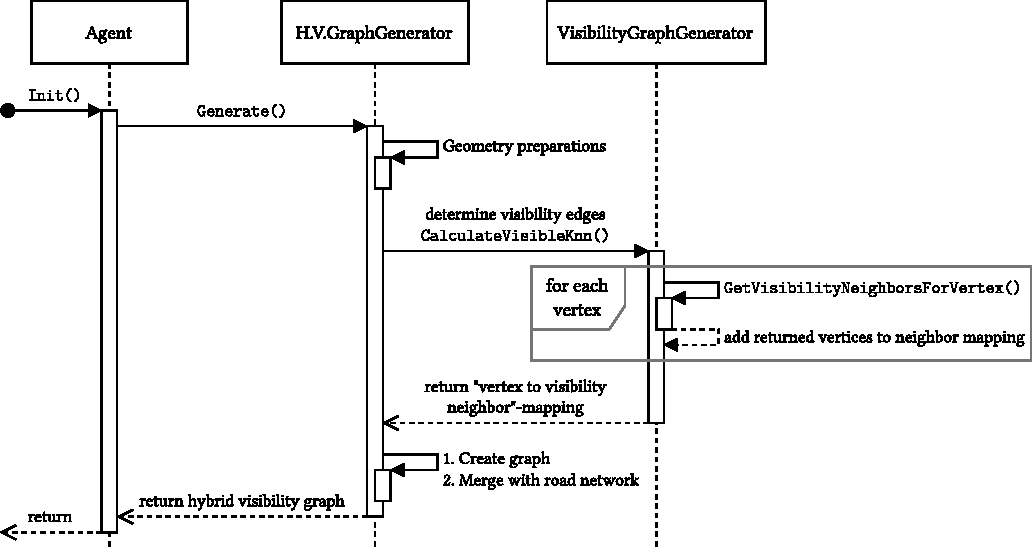
\includegraphics[width=0.98\textwidth]{images/components-sequence-generation-short.pdf}
				\end{figcenter}
				\caption{Separate steps of the graph generation.}
			\end{figure}
		\end{frame}
		
		\begin{frame}{Routing}
			\begin{figure}[t]
				\begin{figcenter}
					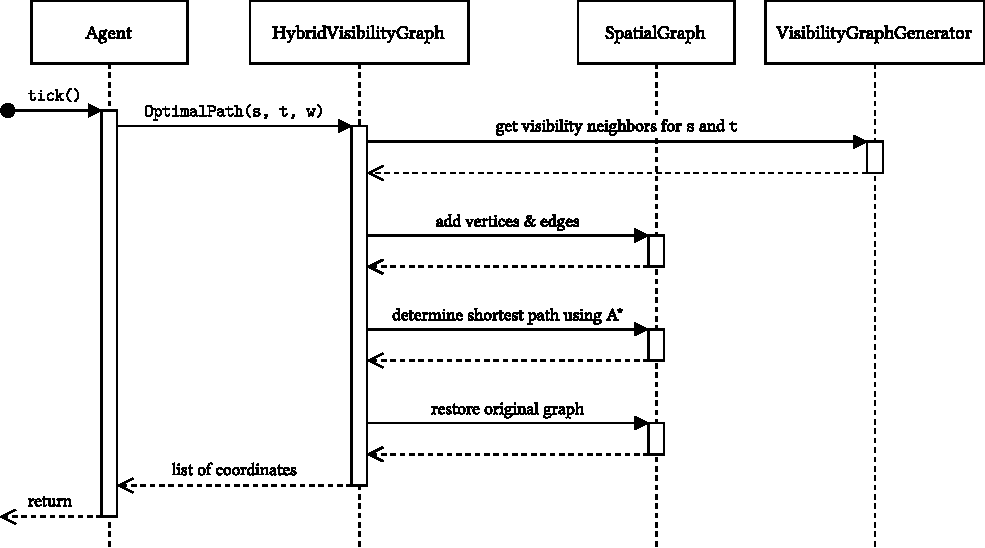
\includegraphics[width=0.95\textwidth]{images/components-sequence-routing-short.pdf}
				\end{figcenter}
				\caption{Separate steps of answering a routing request.}
			\end{figure}
		\end{frame}
	
	\section{Implementation}
	
		\begin{frame}{Considerations and terminology}
			Key considerations:\n
			\begin{itemize}
				\item custom implementation that supports
				\begin{itemize}
					\item collinear vertices
					\item arbitrary obstacle geometries (especially lines and polygons)
					\item intersecting obstacles
					\item arbitrary positions and non-unique coordinates
				\end{itemize}
				\item generate and connect nodes suitable for routing
			\end{itemize}
			\nn
			\pause
			Terminology:\n
			\begin{description}[visibility neighbor]
				\item[obstacle neighbor] vertex on same or touching obstacle
				\item[visibility neighbor] vertex across open space that is visible
				\item[input vertex] vertex / coordinate in the input dataset
				\item[output vertex] generated vertex in the visibility graph
			\end{description}
		\end{frame}
		
		\begin{frame}{Preparations}
			Before visibility graph is created:\n
			\begin{itemize}
				\item get obstacles from input data
				\item unwrap multi-geometries
				\item triangulate polygonal obstacles
				\begin{itemize}
					\item[\textrightarrow] performance optimization
				\end{itemize}
			\end{itemize}
		\end{frame}
		
		\begin{frame}{Visibility graph creation}
			\begin{enumerate}
				\item get obstacles from input data
				\item obtain data for visibility graph
				\begin{enumerate}
					\item for each vertex: determine its visibility neighbors
					\item sort visibility neighbors into bins based on obstacle neighbors
				\end{enumerate}
				\item generate routable visibility graph
				\item merge road edges
			\end{enumerate}
		\end{frame}
		
		\begin{frame}{Visibility graph creation: vertex and edge creation}
			Naive approach:
			\begin{itemize}
				\item one vertex per input coordinate
				\item routing through line-based obstacles possible
			\end{itemize}
			\nn
			\pause
			Correct approach:
			\begin{itemize}
				\item one vertex between adjacent obstacle neighbors
				\item multiple vertices at same location
				\item vertices are not connected
				\item routing through obstacle not possible
			\end{itemize}
		\end{frame}
	
		\begin{frame}{Visibility graph creation: vertex and edge creation}
			\begin{figure}
				\begin{figcenter}
					\scalebox{0.7}
					{
						\begin{tikzpicture}
	\def\d{0.03}
	
	\tikzDot[label=below:$v$]{(0,0)}{v}
	
	\tikzDot[label=left:$n_1$]{(-2.25,0)}{n1}
	\tikzDot[label=above:$n_2$]{(0,2)}{n2}
	\tikzDot[label=right:$n_3$]{(2.25,0)}{n3}
	
	\draw[lightgray] (v) -- (n1);
	\draw[lightgray] (v) -- (n3);
	\draw[lightgray] (v) -- (n2);
	
	% Visibility edges to n1
	\tikzDot[DodgerBlue3]{(-1.1,-0.25)}{vn1}
	\tikzDot[DodgerBlue3]{(-1.6,-0.9)}{vn2}
	\tikzDot[DodgerBlue3]{(1.6,-0.5)}{vn3}
	\draw[DodgerBlue3,densely dashed,->] (v) -- (vn1);
	\draw[DodgerBlue3,densely dashed,->] (v) -- (vn2);
	\draw[DodgerBlue3,densely dashed,->] (v) -- (vn3);
	
	% Visibility edges to n3
	\tikzDot[Red2]{(0.7,1.4)}{vn4}
	\tikzDot[Red2]{(2,1)}{vn5}
	\draw[Red2,densely dotted,->] (v) -- (vn4);
	\draw[Red2,densely dotted,->] (v) -- (vn5);
	
	% Visibility edges to n2
	\tikzDot[Green4]{(-2,1.3)}{vn6}
	\draw[Green4,dashdotted,->] (v) -- (vn6);
\end{tikzpicture}
					}
				\end{figcenter}
				\caption{Sorting visibility neighbors into bins, based on the obstacle neighbors of $v$.}
			\end{figure}
			\pause
			\begin{figure}
				\begin{figcenter}
					\scalebox{0.7}
					{
						\begin{tikzpicture}
	\tikzDot{(2,0)}{vo0};
	\tikzDot[label={[label distance=-1.25mm]above right:$v $}]{(2,1)}{vo1};
	\tikzDot{(2,2)}{vo2};
	
	\draw (vo0) -- (vo1);
	\draw (vo1) -- (vo2);
	
	\tikzDot[label=left:$n_a$,outer sep=0.5mm]{(0.5,1.3)}{n1};
	\tikzDot[label=right:$n_b$,outer sep=0.5mm]{(3.5,1)}{n2};
	
	\draw[dotted] (n1) -- (vo1);
	\draw[dotted] (vo1) -- (n2);
	
	\draw[dotted] (n1) -- (vo0);
	\draw[dotted] (n1) -- (vo2);
	\draw[dotted] (n2) -- (vo0);
	\draw[dotted] (n2) -- (vo2);
\end{tikzpicture}
					}
					\hspace{0.75cm}
					\scalebox{0.7}
					{
						\begin{tikzpicture}
	\def\r{0.85mm}
	\def\rMargin{1.1mm} % = r + 0.25mm
	\def\gap{0.1875mm}
	
	\tikzDot{(2,0)}{vo0};
	\node (vo1) at (2,1) {};
	\node[label={[label distance=-1.25mm]above left:$v_a$}] at (vo1) {};
	\node[label={[label distance=-1.25mm]above right:$v_b$}] at (vo1) {};
	\coordinate (vo11) at ($(vo1)+(180:\rMargin)$);
	\coordinate (vo12) at ($(vo1)+(0:\rMargin)$);
	\tikzDot{(2,2)}{vo2};
	
	\filldraw (vo1)++(-\gap,0)++(90:\r) arc (90:270:\r);
	\filldraw (vo1)++( \gap,0)++(90:\r) arc (90:-90:\r);
	
	\draw ($(vo1)+(270:\r)+(-0.275mm,0)$) -- ($(vo0)+(-0.275mm,2mm)$) -- (vo0.north);
	\draw ($(vo1)+(270:\r)+( 0.275mm,0)$) -- ($(vo0)+( 0.275mm,2mm)$) -- (vo0.north);
	
	\draw ($(vo1)+(90:\r)+(-0.275mm,0)$) -- ($(vo2)+(-0.275mm,-2mm)$) -- (vo2.south);
	\draw ($(vo1)+(90:\r)+( 0.275mm,0)$) -- ($(vo2)+( 0.275mm,-2mm)$) -- (vo2.south);
	
	\tikzDot[label=left:$n_a$,outer sep=0.5mm]{(0.5,1.3)}{n1};
	\tikzDot[label=right:$n_b$,outer sep=0.5mm]{(3.5,1)}{n2};
	
	\draw[dotted] (n1) -- (vo11);
	\draw[dotted] (vo12) -- (n2);
	
	\draw[dotted] (n1) -- (vo0);
	\draw[dotted] (n1) -- (vo2);
	\draw[dotted] (n2) -- (vo0);
	\draw[dotted] (n2) -- (vo2);
\end{tikzpicture}
					}
				\end{figcenter}
				\caption{Naive (left) and correct (right) vertex creation and connection.}
			\end{figure}
		\end{frame}
		
		\begin{frame}{Road network merge}
			\begin{enumerate}
				\item create vertices at intersection points
				\item connect new vertex
				\item remove old edges
			\end{enumerate}
			\begin{figure}
				\begin{figcenter}
					\scalebox{0.7}
					{
						\begin{tikzpicture}
	\tikzDot{(0,-0.75)}{v1n1}
	\tikzDot{(4,-0.6)}{v1n2}
	
	\tikzDot{(0,0.8)}{v2n1}
	\tikzDot{(4.2,0.6)}{v2n2}
	
	\tikzDot{(1.5,-1.65)}{rn1}
	\tikzDot{(1.8,1.65)}{rn2}
	
	\draw[<->,dashed] (v1n1) -- node[above right=0cm and 0.4cm] {$v$} (v1n2);
	\draw[<->,dashed] (v2n1) -- node[above right=0cm and 0.4cm] {$u$} (v2n2);
	
	\draw[<->] (rn1) -- node[left] {$r$} (rn2);
\end{tikzpicture}
					}
					\hspace{0.75cm}
					\scalebox{0.7}
					{
						\begin{tikzpicture}
	\tikzDot{(0,-0.75)}{v1n1}
	\tikzDot{(4,-0.6)}{v1n2}
	
	\tikzDot{(0,0.8)}{v2n1}
	\tikzDot{(4.2,0.6)}{v2n2}
	
	\tikzDot{(1.5,-1.65)}{rn1}
	\tikzDot{(1.8,1.65)}{rn2}
	
	\tikzDot{(intersection of v1n1--v1n2 and rn1--rn2)}{i1}
	\tikzDot{(intersection of v2n1--v2n2 and rn1--rn2)}{i2}
	
	\draw[<->,dashed] (v1n1) -- node[above] {$v_1$} (i1);
	\draw[<->,dashed] (i1)   -- node[above] {$v_2$} (v1n2);
	\draw[<->,dashed] (v2n1) -- node[above] {$u_1$} (i2);
	\draw[<->,dashed] (i2)   -- node[above] {$u_2$} (v2n2);
	
	\draw[<->] (rn1) -- node[right] {$r_1$} (i1);
	\draw[<->] (i1)  -- node[right] {$r_2$} (i2);
	\draw[<->] (i2)  -- node[right] {$r_3$} (rn2);
\end{tikzpicture}
					}
				\end{figcenter}
				\caption{Merge of road network and visibility edges.}
			\end{figure}
		\end{frame}
		
		\begin{frame}{Answering routing queries}
			\begin{enumerate}
				\item add vertices for source \& destination to graph
				\item create and add their visibility edges
				\begin{itemize}
					\item[\textrightarrow] same algorithm used for graph generation
				\end{itemize}
				\item use A* to determine shortest path
				\item remove previously created vertices and edges
			\end{enumerate}
		\end{frame}
		
		\begin{frame}{Performance optimizations}
			Only consider $k = k_b \cdot k_n$ many visibility neighbors:
			\begin{itemize}
				\item ensure neighbors exist in all directions
				\item $k_b$ bins, each covering $360 / k_b$ degree
				\item $k_n$ neighbors per bin
			\end{itemize}
			\nn
			\pause
			Only consider vertices on a convex hull:\n
			\begin{itemize}
				\item convex hull is shortest path around polygon
				\item[\textrightarrow\hspace{-0.1cm}] vertex not on any convex hull will never be part of any shortest path
			\end{itemize}
		\end{frame}
		
		\begin{frame}{Performance optimizations}
			Only consider potential visibility neighbors at certain angles:\n
			\begin{itemize}
				\item consider shortest path $p$\ \textrightarrow\ no edges can be relaxed
				\item only vertices at certain angles are valid neighbors\ \textrightarrow\ valid angle area
			\end{itemize}
			\pause
			\begin{figure}[b]
				\begin{figcenter}
					\scalebox{0.7}
					{
						\begin{tikzpicture}
	\coordinate (c00) at (0,0.4);
	\draw (c00)
	-- ++(2.75,-0.2) coordinate (c01)
	-- ++(0.8,0.4) coordinate (c02)
	-- ++(0.1,0.8) coordinate (c03)
	-- ++(-2,0) coordinate (c04)
	-- ++(-1.4,-0.35) coordinate (c05)
	-- (c00);
	\node[above right = 0.15 and 1.6 of c00] {$o_1$};
	
	\coordinate (c10) at (2.5,3.85);
	\draw (c10)
	-- ++(-0.4,-0.4) coordinate (c11)
	-- ++(0.1,-0.6) coordinate (c12)
	-- ++(2.8,0) coordinate (c13)
	-- ++(-0.4,1.2) coordinate (c14)
	-- (c10);
	\node[below right = 0.25 and 0.75 of c10] {$o_2$};
	
	\def\d{1.5\pgflinewidth}
	\filldraw[line width=0,Green4!35!white]
	($(c03)+(0,\d)$) --
	+(180:0.35) arc [start angle=180, delta angle=-97.126, radius=0.35];
	\draw[thin,Green4] (c03) -- (intersection of c03--[shift=(c03)]82.874:3 and c12--c13);
	\draw[thin,Green4] ($(c03)+(0,\d)$) -- +(180:4);
	
	\filldraw[line width=0,DodgerBlue3!35!white]
	($(c12)+(0,-\d)$) --
	+(279.462:0.4) arc [start angle=279.462, delta angle=80.538, radius=0.4];
	\draw[thin,DodgerBlue3] (c12) -- (intersection of c12--[shift=(c12)]279.462:1 and c03--c04);
	\draw[thin,DodgerBlue3] ($(c12)+(0,-\d)$) -- +(0:4);
	
	\tikzDot[label={right:$s$}]{(c01)}{s}
	\tikzDot[label={right:$v_0$}]{(c02)}{v0}
	\tikzDot[label={right:$v_1$}]{(c03)}{v1}
	\tikzDot[label={left:$v_2$}]{(c12)}{v2}
	\tikzDot[label={below:$v_3$}]{(c13)}{v3}
	\tikzDot[label={above:$v_4$}]{(c04)}{v4}
	\tikzDot[label={left:$t$}]{(c10)}{t}
	
	\draw[->,Red2,thick] (s) -- (v0);
	\draw[->,Red2,thick] (v0) -- (v1);
	\draw[->,Red2,thick] (v1) -- (v2);
	\draw[->,Red2,thick] (v2) -- (c11);
	\draw[->,Red2,thick] (c11) -- (t);
\end{tikzpicture}

					}
				\end{figcenter}
				\caption{Valid angle areas (blue and green).}
			\end{figure}
		\end{frame}
		
		\begin{frame}{Performance optimizations}
			Exclude vertices in \enquote{shadow} of obstacles:\n
			\begin{itemize}
				\item consider vertex $v$ and think of it as light bulb
				\item obstacles cast shadow outwards, hiding vertices
			\end{itemize}
			\pause
			\begin{figure}[b]
				\begin{figcenter}
					\scalebox{0.7}
					{
						\begin{tikzpicture}
	\def\angle{20}
	\def\boundingVertexDistance{3}
	
	\tikzDot[label=$v$]{(0,1.5)}{v}
	\coordinate (shadow-arc-top)				at ($(v) +( \angle:\boundingVertexDistance)$);
	\coordinate (shadow-arc-bottom)				at ($(v) +(-\angle:\boundingVertexDistance)$);
	\coordinate (shadow-arc-top-end)			at ($(v) +( \angle:5.75)$);
	\coordinate (shadow-arc-bottom-end)			at ($(v) +(-\angle:5.75)$);
	\coordinate (shadow-arc-top-faded-end)		at ($(v) +( \angle:6.5)$);
	\coordinate (shadow-arc-bottom-faded-end)	at ($(v) +(-\angle:6.5)$);
	
	% Gray area
	\filldraw[lightgray] 
	(shadow-arc-bottom) arc [start angle=-\angle, delta angle=2*\angle, radius=\boundingVertexDistance] --
	(shadow-arc-top-end) --
	(shadow-arc-bottom-end) --
	cycle;
	\draw[gray]
	(shadow-arc-bottom-end) --
	(shadow-arc-bottom) arc [start angle=-\angle, delta angle=2*\angle, radius=\boundingVertexDistance] --
	(shadow-arc-top-end);
	
	\draw[dotted] (v) -- (shadow-arc-top);
	\draw[dotted] (v) -- (shadow-arc-bottom);
	
	% Faded gray area
	\filldraw[draw=none,lightgray,path fading=east]
	(shadow-arc-top-faded-end) --
	(shadow-arc-top-end) --
	(shadow-arc-bottom-end) --
	(shadow-arc-bottom-faded-end) --
	cycle;
	\draw[gray,path fading=east] (shadow-arc-top-end) -- (shadow-arc-top-faded-end);
	\draw[gray,path fading=east] (shadow-arc-bottom-end) -- (shadow-arc-bottom-faded-end);
	
	% Obstacle
	\tikzDot[Red2]{(shadow-arc-top)}{o0}
	\tikzDot{(3.8,2)}{o1}
	\tikzDot[Red2]{($(v) +(-\angle:1.2)$)}{o2}
	\node[above right = 0.5 and 1.15 of o2] {$o$};
	
	% v' and v''
	\tikzDot[label=right:$v'$]{(2.1,1.1)}{v'}
	\tikzDot[label=right:$v''$]{(3.4,1.3)}{v''}
	
	\node[darkgray] at (4.7,1.5) {\huge$S$};
	
	\draw (o0) -- (o1) -- (o2) -- (o0);
\end{tikzpicture}

					}
				\end{figcenter}
				\caption{Shadow area $S$ cast by obstacle $o$.}
			\end{figure}
		\end{frame}
		
		\begin{frame}{Performance optimizations}
			Interval data structure for shadow areas:\n
			\begin{itemize}
				\item bin-based: each bin covers certain angle interval
				\item constant-time bin access
			\end{itemize}
			\pause
			\begin{figure}[b]
				\begin{figcenter}
					\scalebox{0.7}
					{
						
\begin{tikzpicture}
	\def\l{0.5}
	\def\countX{9} % One more is added due to start at x=0
	\def\countY{1} % One more is added due to start at x=0
	
	\def\itemBStartX{1.6}
	\def\itemBIndexStart{1}
	\def\itemBLength{4.1}
	
	\def\itemAStartX{4}
	\def\itemAIndexStart{4}
	\def\itemALength{7.8}
	
	% Item A: Bins 1-5
	\draw[dotted,gray] (\itemBStartX*\l, \countY+4*\l) -- +(0, -\countY-4*\l);
	\draw[dotted,gray] (\itemBStartX*\l+\itemBLength*\l, \countY+4*\l) -- +(0, -\countY-4*\l);
	\filldraw[preaction={fill, white},pattern=north west lines,pattern color=Red2] (\itemBStartX*\l,\countY+4*\l) rectangle node[above right=0.125 and -1.3]{Item B: \itemBStartX\ - 5.7} ++(\itemBLength*\l,0.5*\l);
	
	% Item B: Bins 4-11(2)
	\draw[dotted,gray] (\itemAStartX*\l, \countY+3*\l) -- +(0, -\countY-3*\l);
	\draw[dotted,gray] (\itemAStartX*\l+\itemALength*\l, \countY+3*\l) -- +(0, -\countY-3*\l);
	\filldraw[preaction={fill, white},pattern=crosshatch dots,pattern color=DodgerBlue3] (\itemAStartX*\l,\countY+3*\l) rectangle node[above right=0.125 and -0.5]{Item A: \itemAStartX\ - 10.8} ++(\itemALength*\l,0.5*\l);
	
	\draw[->] (\itemAStartX*\l+1.85,\countY+2.75*\l) -- node[right] {1.} +(0,-1.5*\l);
	\draw[->] (\itemBStartX*\l+0.5,\countY+3.75*\l) -- node[right] {2.} +(0,-2.5*\l);
	
	% Draw pattern to bins
	\fill[preaction={fill, white},pattern=north west lines,pattern color=Red2] (\itemBIndexStart*\l,1.5*\l) rectangle ++(\l,\l);
	\fill[preaction={fill, white},pattern=north west lines,pattern color=Red2] (\itemBIndexStart*\l+1*\l,0) rectangle ++(2*\l,\l);
	\fill[preaction={fill, white},pattern=north west lines,pattern color=Red2] (\itemBIndexStart*\l+3*\l,1.5*\l) rectangle ++(\l,\l);
	\fill[preaction={fill, white},pattern=north west lines,pattern color=Red2] (\itemBIndexStart*\l+4*\l,1.5*\l) rectangle ++(\l,\l);
	
	\fill[preaction={fill, white},pattern=crosshatch dots,pattern color=DodgerBlue3] (\itemAIndexStart*\l,0) rectangle ++(6*\l,\l);
	\fill[preaction={fill, white},pattern=crosshatch dots,pattern color=DodgerBlue3] (0,0) rectangle ++(2*\l,\l);
	
	% Draw gray versions of filled bins
	\fill[preaction={fill, white},pattern=north west lines,pattern color=lightgray] (\l*\countX+\l+\itemBIndexStart*\l+1*\l,0) rectangle ++(\l,\l);
	\fill[preaction={fill, white},pattern=crosshatch dots,pattern color=lightgray] (\l*\countX+\l,0) rectangle ++(2*\l,\l);
	
	% Draw outlines of repeating gray bins
	\foreach \x in {0,...,2}
	{
		\draw[lightgray] (\l*\countX+\l+\l*\x,0) rectangle ++(\l,\l);
		\node[lightgray] at (\l*\countX+\l+\l*\x+0.5*\l,-0.35) {$\x$};
	}
	
	% Draw outlines of bins
	\foreach \x in {0,...,\countX}
	{
		\draw (\l*\x,0) rectangle ++(\l,\l);
		\node at (\l*\x+0.5*\l,-0.35) {$\x$};
	}
	
	\draw (\itemBIndexStart*\l,1.5*\l) rectangle ++(\l,\l);
	\draw[->] (\itemBIndexStart*\l+0.5*\l,\l) -- ++(0,0.5*\l);
	
	\draw (\itemBIndexStart*\l+3*\l,1.5*\l) rectangle ++(\l,\l);
	\draw[->] (\itemBIndexStart*\l+3.5*\l,\l) -- ++(0,0.5*\l);
	
	\draw (\itemBIndexStart*\l+4*\l,1.5*\l) rectangle ++(\l,\l);
	\draw[->] (\itemBIndexStart*\l+4.5*\l,\l) -- ++(0,0.5*\l);
	
	\node at (0.5*\countX*\l,-0.875) {bins};
	\node[align=right] at (-1.25,0.5*\countY*\l+0.5*\l) {Linked lists\\of bins};
\end{tikzpicture}
					}
				\end{figcenter}
				\caption{BinIndex data structure storing two overlapping intervals.}
			\end{figure}
		\end{frame}
		
		\begin{frame}{Performance optimizations}
			Additional optimizations:
			\begin{itemize}
				\item usage of spatial indices
				\item custom line segment intersection check
				\item custom triangle intersection check
			\end{itemize}
		\end{frame}
	
	\section{Evaluation}
	
	\section{Conclusion}
\end{document}